Here are the distances computed by the cosine metric with the TF-IDF terms:
\begin{figure}[H]
    \begin{minipage}[b]{0.3\linewidth}
        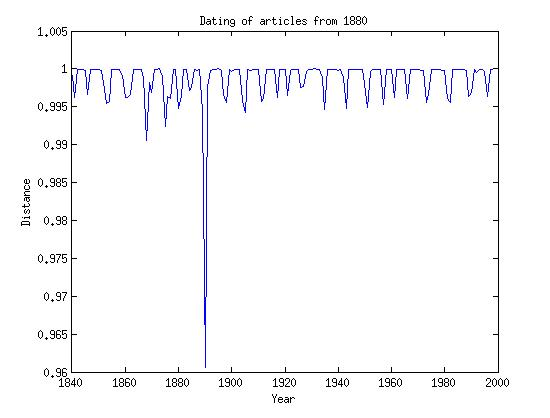
\includegraphics[scale=0.25]{Pictures/date_articles/cos/dating1880_tfidf.jpg}
        \caption{Dating articles from 1880 with the cosine distance with TF-IDF. Prediction is 1890.}
    \end{minipage}\hfill
    \begin{minipage}[b]{0.3\linewidth}
        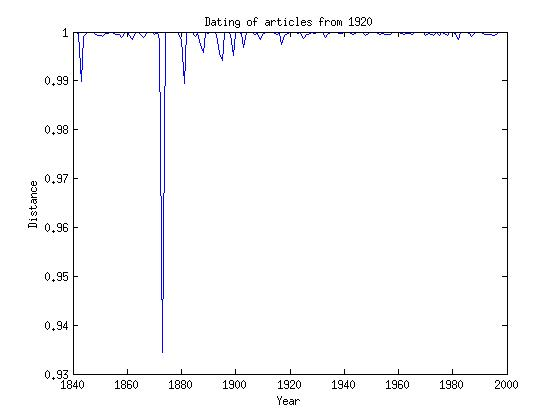
\includegraphics[scale=0.25]{Pictures/date_articles/cos/dating1920_tfidf.jpg}
        \caption{Dating articles from 1920 with the cosine distance with TF-IDF. Prediction is 1873.}
    \end{minipage}\hfill
    \begin{minipage}[b]{0.3\linewidth}
	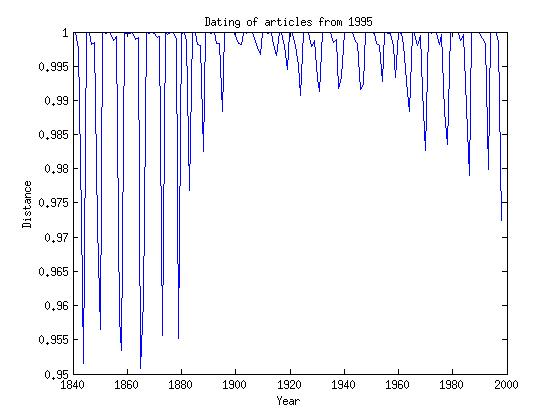
\includegraphics[scale=0.25]{Pictures/date_articles/cos/dating1995_tfidf.jpg}
        \caption{Dating articles from 1995 with the cosine distance with TF-IDF. Prediction is 1865.}
        \label{date_cos_tfidf1}
    \end{minipage}
\end{figure}

The prediction is much more precise than with the previous metrics. As we saw in figure \ref{cos_tfidf}, low distances are very close to the diagonal which means that $d(year1, year2)$ is lower than $1$ only if $year1$ and $year2$ are close to each other. With this property, the prediction of the cosine metric with TF-IDF terms will often be very close to the real year of the articles.